\chapter{Independent Component Analysis(ICA)}

ICA tries to find original signals $\hat{S}$. from mixed signal $X$, called Blind Source Separation problem.
$$
X = AS \hspace{1cm}  \rightarrow \hspace{1cm} \hat{S}  = WX
$$
where 

\begin{itemize}
	\item $X \in \mathbb{R}^{\text{Nxp}}$
	\item $A, W \in \mathbb{R}^{\text{NxN}}$
	\item $S, \hat{S} \in \mathbb{R}^{\text{Nxp}}$
	\item $N$ is no. sources
	\item $p$ is no. observations in the source
\end{itemize}

One could say that ICA tries to find $W \approx A^{-1}$.

\section{ICA vs PCA}

The goal of PCA is to find directions that don't correlate with each other( orthogonal projections ). However, ICA finds sources that are independent to each other.  The right most figure of Fig \ref{fig:ica-decorrleation-vs-independent} shows that even correlation$C_{12}, C_{21}$ is zero, but $x_1, x_2$ are dependent to each other( knowing one of them can tell position of the other ).

\begin{figure}[hbt]
	\center
  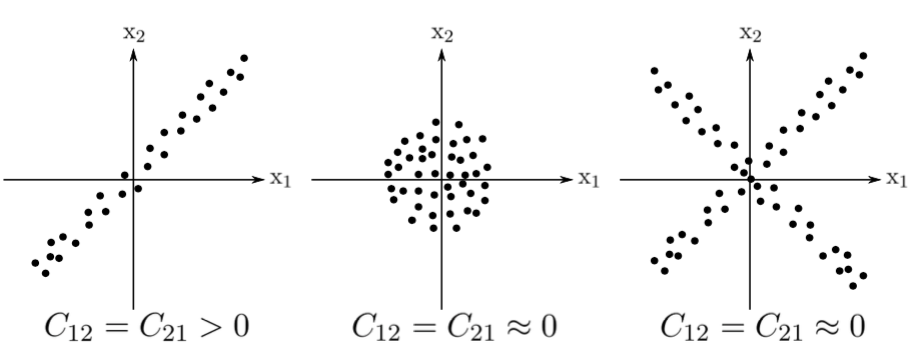
\includegraphics[width=0.8\textwidth]{figures/ica-decorrelation-vs-indepedent}
  \caption{Decorrelation vs Indenpendent (Drawn from MI2 Slides)}
  \label{fig:ica-decorrleation-vs-independent}
\end{figure}

\section{ICA Limitations}
\subsection{Permutation of Sources}
$\boldsymbol{\hat{s}}_i$ that found that ICA is not necessary the same as the original source $\boldsymbol{s}_i$.
\subsection{Discovered Amplitude}
\subsection{Gaussian Sources}
The underly theory behind ICA is Central Limit Theorem in which it implies that  sum of random variables will approach Gaussian distribution. Thus, if the original sources come from Gaussian distribution, we won't have any clue to separate the sources.


\section{ICA Approaches}
An ICA algorithm can be derived using different cost functions using assumption that 
\begin{align*}
	\hat{P}_{\boldsymbol{s}}(\boldsymbol{\hat{s}}) = \prod_{i=1}^N \hat{P}_{s_i}(\hat{s}_i)
\end{align*}

and ${P}_{\boldsymbol{s}}(\boldsymbol{\hat{s}}) = P_{\boldsymbol{s}}(W\boldsymbol{x})$

\subsection{Informax}
From Kullback-Leibler divergence, we know that 

\begin{align*}
D_{KL}(P||Q) = \int_{-\infty}^{\infty}  p(x) \log \frac{ p(x) } { q(x) } dx	
\end{align*}

Thus, we can formulate the problem as
\begin{align*}
\min_{W} D_{KL} ( P_{\boldsymbol{s}}(\boldsymbol{\hat{s}}) || \hat{P}_{\boldsymbol{s}}(\boldsymbol{\hat{s}}) )
\end{align*}

However, deriving cost from $D_{KL}$ directly would not work as it require probability density estimation. Hence, we shall use a transformation :
\begin{align*}
	\hat{u}_i = \hat{f}( \hat{s}_i ) \hspace{1cm} \text{s.t.} \hspace{1cm}  \hat{P}_{u_i}(\hat{u}_i) = \text{const.}
\end{align*}

From Conservation of Probability, we know that 
\begin{align*}
	\hat{P}_{u_i}(\hat{u}_i) d\hat{u}_i =\hat{P}_{s_i}(\hat{s}_i) d\hat{s}_i
\end{align*}

Then
\begin{align*}
	\hat{P}_{u_i} &= \Bigg |  \frac{d\hat{s}_i}{d\hat{u}_i} \Bigg | \hat{P}_{s_i}(\hat{s}_i)  \\
	&= \Bigg |  \frac{1}{\frac{d\hat{u}_i}{d\hat{s}_i}} \Bigg | \hat{P}_{s_i}(\hat{s}_i) \\
	&= \Bigg |  \frac{1}{ \hat{f}'( \hat{s}_i )  } \Bigg | \hat{P}_{s_i}(\hat{s}_i) \\
	&\stackrel{!}{=}1
\end{align*}

This implies that $\hat{f}({\hat{s}_i})$ is CDF of $\hat{P}_{s_i}(\hat{s}_i)$. From this knowledge, we can derive $D_{KL}$ :

\begin{align*}
	 D_{KL} ( P_{\boldsymbol{s}}(\boldsymbol{\hat{s}}) || \hat{P}_{\boldsymbol{s}}(\boldsymbol{\hat{s}}) ) &= \int_{-\infty}^{\infty} d\boldsymbol{\hat{s}} P_{\boldsymbol{s}} (\boldsymbol{\hat{s}}) \log \frac{ P_{\boldsymbol{s}}(\boldsymbol{\hat{s}}) }{
	 	\prod_{i=1}^{N} \hat{P}_{s_i}(\hat{s}_i)
	 	}  \\
	 	&= \int_{-\infty}^{\infty} d\boldsymbol{\hat{s}} P_{\boldsymbol{s}} (\boldsymbol{\hat{s}}) \log \frac{ P_{\boldsymbol{s}}(\boldsymbol{\hat{s}}) }{
	 	\prod_{i=1}^{N} \hat{P}_{s_i}(\hat{s}_i)
	 	}  \frac{ \prod_{i=1}^{N} 1/\hat{f}' }{ \prod_{i=1}^{N} 1/\hat{f}'  } \\
	 	&= \int_{-\infty}^{\infty} d\boldsymbol{\hat{u}} P_{\boldsymbol{u}} (\boldsymbol{\hat{u}}) \log \frac{ P_{\boldsymbol{u}}(\boldsymbol{\hat{u}}) }{
	 	\prod_{i=1}^{N} \hat{P}_{u_i}(\hat{u}_i)
	 	}  \\
	 	&= \int_{-\infty}^{\infty} d\boldsymbol{\hat{u}} P_{\boldsymbol{u}} (\boldsymbol{\hat{u}}) \log  P_{\boldsymbol{u}}(\boldsymbol{\hat{u}}) 
	 	- 	 	
	 	\int_{-\infty}^{\infty} d\boldsymbol{\hat{u}} P_{\boldsymbol{u}} (\boldsymbol{\hat{u}})
	 	\log \prod_{i=1}^{N} \hat{P}_{u_i}(\hat{u}_i)
	 	  \\
\end{align*}

Hence, 
\begin{align*}
	\min D_{KL} ( P_{\boldsymbol{s}}(\boldsymbol{\hat{s}}) || \hat{P}_{\boldsymbol{s}}(\boldsymbol{\hat{s}}) ) &\approx \min  \int_{-\infty}^{\infty} d\boldsymbol{\hat{u}} P_{\boldsymbol{u}} (\boldsymbol{\hat{u}}) \log  P_{\boldsymbol{u}}(\boldsymbol{\hat{u}})  \\
		& \approx \min -H(u) \\
		& \approx \max H(u) \tag*{(Informax Principle)}
\end{align*}

\subsubsection{Learning via Neural Network and Empirical Risk Minimization} 
From Conservation of Probability, we know that 
\begin{align*}
	 P(\boldsymbol{\hat{u}})d\boldsymbol{\hat{u}} &= P(\boldsymbol{\hat{s}})d\boldsymbol{\hat{s}} \\ 
	 &= P(\boldsymbol{x})d\boldsymbol{x} 
\end{align*}
and, 
\begin{align*}
	 \boldsymbol{\hat{u}} &= \hat{f}(\boldsymbol{\hat{s}}) \\
	 &= \hat{f}(W\boldsymbol{{x}})
\end{align*}

Thus, 
\begin{align*}
		 P(\boldsymbol{\hat{u}})  &=  P(\boldsymbol{x})d\boldsymbol{x} 
\\
&=  \Bigg | \frac{d\boldsymbol{x}}{d\boldsymbol{\hat{u}}} \Bigg | P(\boldsymbol{x}) \\
&=   \frac{1}{|M|} P(\boldsymbol{x}) 
\end{align*}
where $|M|$ is functional determinant and 
\begin{align*}
|M| &= \Bigg| \frac{\partial \boldsymbol{\hat{u}}}{ \partial \boldsymbol{x}}\Bigg|	\\
&= |W| \prod_{l=1}^{N} \hat{f}' \bigg (\sum_{k=1}^{N} w_{lk}x_k \bigg )
\end{align*}

Hence,
\begin{align*}
	H(\boldsymbol{u}) &= - \int d\boldsymbol{\hat{u}} P_{\boldsymbol{u}}(\boldsymbol{\hat{
	u}})\log P_{\boldsymbol{u}}(\boldsymbol{\hat{
	u}}) \\
	&= - \int d\boldsymbol{x} P_{\boldsymbol{x}}(\boldsymbol{x})\log \frac{P_{\boldsymbol{x}}(\boldsymbol{\hat{x}}}{|M|}) \\
	&= - \int d\boldsymbol{x} P_{\boldsymbol{x}}(\boldsymbol{x})\log P_{\boldsymbol{x}} +
	\int d\boldsymbol{x} P_{\boldsymbol{x}}(\boldsymbol{x})\log |M| 
\end{align*}

Because $- \int d\boldsymbol{x} P_{\boldsymbol{x}}(\boldsymbol{x})\log P_{\boldsymbol{x}}$ is a constant if we optimize over $w$, therefore, the cost function $E^G$ is reduced to 
\begin{align*}
	E^G &= 	\ 	\int d\boldsymbol{x} P_{\boldsymbol{x}}(\boldsymbol{x})\log |M| \\
	&= 	\int d\boldsymbol{x} P_{\boldsymbol{x}}(\boldsymbol{x})\log |W| + 	\int d \boldsymbol{x} P_{\boldsymbol{x}}(\boldsymbol{x})\log  \prod_{l=1}^{N} \hat{f}' \bigg (\sum_{k=1}^{N} w_{lk}x_k \bigg ) \\
	&= \log |W| + \int d \boldsymbol{x} P_{\boldsymbol{x}}(\boldsymbol{x}) \Bigg\{ \sum_{l=1}^{N} \log\hat{f}'\bigg (\sum_{k=1}^{N} w_{lk}x_k \bigg ) \Bigg\}
\end{align*}

Using Empirical Risk Minimization, we convert expectation to average  thus 

\begin{align*}
	E^T &= \log |W| + 
	\frac{1}{p} \sum_{\alpha=1}^{p} \sum_{l=1}^{N} \log\hat{f} ' \bigg (\sum_{k=1}^{N} w_{lk}x_k^{(\alpha)} \bigg )  \\
	&\stackrel{!}{=} \max_{W}
\end{align*}

We can learn $W$ using gradient ascent :
\begin{align*}
  W \leftarrow W + \eta \nabla_{W} E^T
\end{align*}

For individual cost of each observation $e^{(\alpha)}$, 
\begin{align*}
	\frac{\partial e^{(\alpha)} }{\partial w_{ij} } &= W ^{-1}_{ji} + \frac{\hat{f} '' \bigg (\sum_{k=1}^{N} w_{ik}x_k^{(\alpha)} \bigg )}{\hat{f} ' \bigg (\sum_{k=1}^{N} w_{ik}x_k^{(\alpha)} \bigg ) } x_j^{(\alpha)}
\end{align*}

Or
\begin{align*}
 \frac{ \partial }{\partial W} e^{(\alpha)} = 	(W^{-1})^T + \psi(Wx^{(\alpha)}) (x^{(\alpha)})^T
\end{align*}


One could observe that there is $W^{-1}$ in the computation which causes performance. 
\subsubsection{Learning via Natural Gradient}
Due to the fact that $W$ space is not  orthogonal coordinate, hence gradient doest point to the direction of steepest ascent. Thus, we need to transform the space back to comparable space before computing gradient. This yields 

\begin{align*}
	dZ = dW \cdot W^{-1}
\end{align*}

Using Taylor expansion of $e^{(\alpha)}$ or $e$ for short, around $W$,  we have :
\begin{align*}
	e( W + dW ) &= e(W) + \nabla_{W} e^T dW  \\
	&=  e(W) + \eta \nabla_{W} e^T z_w
\end{align*}

where $z_w = \eta dw$

To find the direction of steepest ascent, we have to 
\begin{align*}
		 \nabla_{W} e^T z_w \stackrel{!}{=} \max \hspace{1cm} \text{s.t.} \hspace{1cm} (z_w \cdot  W^{-1} )^2 \stackrel{!}{=} 1
\end{align*}

Using Lagrange multiplier we have 

\begin{align*}
	\mathcal{L}(z_w, \lambda)  =  \nabla_{W} e^T z_w - \lambda ( (z_w \cdot  W^{-1} )^2 - 1 )
\end{align*}

Taking derivative wrt to $z_w$ and set to zero, we have 
\begin{align*}
  0 &= \nabla_{W} e - 2\lambda ( z_w \cdot W^{-1} )(W^{-1})^T \\
    \nabla_{W} e &= 2\lambda ( z_w \cdot W^{-1} )(W^{-1})^T \\
    z_w &= \frac{1}{2\lambda} \nabla_{W} e W^T W
\end{align*} 

Hence the direction for \textbf{Natural Gradient} is 
\begin{align*}
	\Delta W = \eta \nabla_{W} e W^T W
\end{align*}

where $\nabla_{W} e$ is original gradient. 

Putting things together, we have 
\begin{align*}
	\Delta W = \eta \Bigg (  \mathbb{I} + \psi(Wx) (Wx)^T \Bigg) W	
\end{align*} 

Commonly, people use the sigmoid function as CDF : 
$$
f(x) = \frac{1}{1+\exp(-x)}  \hspace{1cm} \rightarrow \hspace{1cm}  \psi(x) = \frac{f''(x)}{f'(x)} = 1 - 2f(x)
$$

\subsection{Second-order Approach}
Due to the fact that, higher moment measurements are sensitive to noise, especially when we have small set of samples, hence it might yield unreliable result. Moreover, signals, such as EEG, fMRI data, might correlate to each other in temporal pattern. Because most of the time we know the length of the signal, we can exploit this fact by using autocorrelation.


Formally, the motivation of 2nd order approach is to find unmixing matrix $W$ that cross-correlation varnishes.
\begin{figure}[hbt]
	\center
  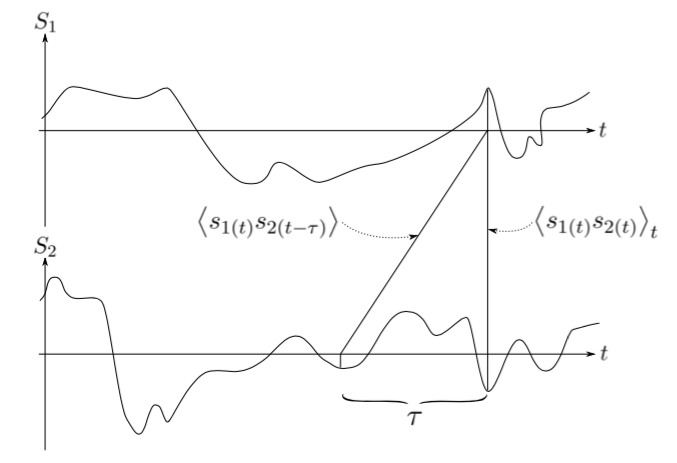
\includegraphics[width=0.8\textwidth]{figures/ica-autocorrelation}
  \caption{Autocorrelation with time $\tau$ shifted (Drawn from MI2 Slides)}
  \label{fig:ica-autocorrelation}
\end{figure}


\subsubsection{Source Separation with 2 shifts}
\begin{enumerate}
	\item  Whitening data 
	\begin{align*}
		\boldsymbol{x}_c = \boldsymbol{x} - \frac{1}{p} \sum_{\alpha} x^{(\alpha)}
	\end{align*}
	Then compute eigen value decomposition of $C_x^{(0)}$ where $(C_x)_{ij} = <x_i, x_j>$. Hence,
	\begin{align*}
		\boldsymbol{u} &= \Lambda_0^{-1/2}  \cdot E_0 \boldsymbol{x} \\
		&= M_0 \boldsymbol{x}
	\end{align*}
	where $\Lambda_0^{-1/2}$ is a diagonal of inverse eigen values and and $E_0$ is matrix of eigen vectors.
	\item Orthogonal Transformation

	Assume : $\boldsymbol{s} = B\boldsymbol{u}$. We know that 
	\begin{align*}
		<s_is_j> &= \delta_{ij} \\
		&= \sum_{k,l=1}^{N}B_{ik}<u_ku_l>B_{l,j}^{T} \\
		&= \sum_{k,l=1}^{N}B_{ik} B_{l,j}^{T} \tag*{($<u_ku_l> = 1 $ from Whitening)} 
	\end{align*} 
	Hence, $$BB^T  = B^TB = \mathbb{I} \leadsto \textbf{Orthogonal Transformation}$$
	
	\item Find a candidate of $B$ using time-shifted cross-correlation matrix
	Apply eigen value decomposition  on $C_u^{(\tau)}$ where 
	$$(C_u^{(\tau)})_{ij} = <u_i^{(t)} u_j^{(t-\tau)} >$$
	This results in a matrix of eigen vectors $E_{\tau}$ whose $E_{\tau}^TE_\tau = \mathbb{I}$ 
	Putthing thing together, we have 
	\begin{align*}
		\boldsymbol{\hat{s}} = E_\tau \Lambda_0^{-1}  E_0 \boldsymbol{x}
	\end{align*}
\end{enumerate}

\subsubsection{Noise robust algorithms in general case}
Given a set of $T$ zero mean observation : $\boldsymbol{x^{(t)}}$. We compute joint cross-correlation metric $C_x^{(\tau)}$ as :
\begin{align*}
(C_x^{(\tau)})_{ij} = \frac{1}{T}	\sum_{t=0}^{T-1}  x_i^{(t)} x_j^{(t-\tau)}
\end{align*}

To find $NxN$ matrix $W$ that diagonalize $C^{(\tau)}, \tau = 0,1, ...$, we use sum of off-diagonal entries of $WC^{(\tau)}W^T$ as a cost function.

\begin{enumerate}
	\item QDIAG Algorithm 
	\begin{align*}
		E^T_{W} = \sum_{\tau} \alpha_\tau \sum_{i \ne j}  \Bigg(  WC^{(\tau)}W^T \Bigg)_{ij}^2
	\end{align*}
	where $\alpha_\tau$ is a weighting factor and the optmization problem is $E^T \stackrel{!}{=} \min$ s.t. 
	$$
\forall i,  \hspace{0.5cm}	\Bigg(  WC^{(0)}W^T \Bigg)_{ii} = 1
	$$
	
	\item FFDIAG Algorithm 
	\begin{align*}
		E^T_{W} = \sum_{\tau}  \sum_{i \ne j}  \Bigg(  WC^{(\tau)}W^T \Bigg)_{ij}^2
	\end{align*}
	with a constraint that $W$ is a non-singular matrix.
\end{enumerate}


\subsection{Maximize Non-Gaussianity}
According to Central Limit Theorem, the sum of random variables is more Gaussian than the original sources. Hence, we can leverage this knowledge by finding a unmixing matrix that minimizes Gaussianity of the unmixed sources yielding interesting directions ( projection pursuit).  There are 2 ways to measure Gaussianity, namely Kurtosis ( 4th moment ) and Negentropy.

\subsubsection{Kurtosis}

\begin{align*}
	\text{kurt}(x) =   \langle x^4 \rangle - 3 \underbrace{ ( \langle x^2 \rangle ) ^2  }_{  \substack{ \text{1 for} \\ \text{sphered data} } }
\end{align*}

\begin{figure}[hbt]
	\center
  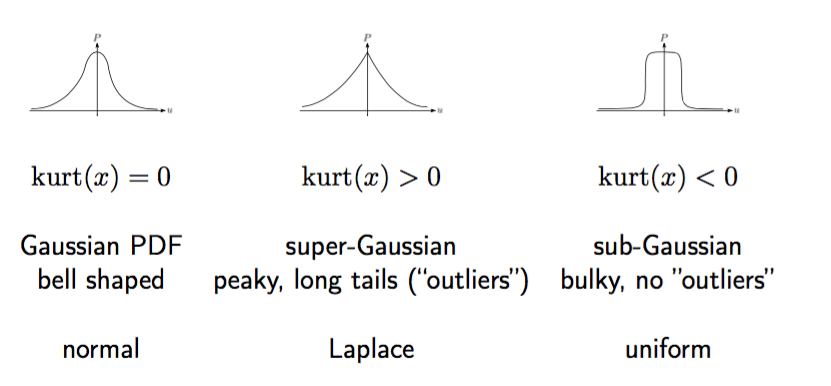
\includegraphics[width=0.5\textwidth]{figures/ica-kurtosis}
  \caption{Distribution and Kurtosis (Drawn from MI2 Slides)}
  \label{fig:ica-kurtosis}
\end{figure}

$\bullet$ $\text{kurt}(x) = 0$  for Gaussian distribution

$\bullet$ $\text{kurt}(x) > 0$ for \textbf{Super}-Gaussian : long-tail, e.g. Laplace Distribution

$\bullet$ $\text{kurt}(x) < 0$ for \textbf{Sub}-Gaussian : constant distribution.


For independent variable $x$ and $y$ we have :
\begin{align*}
	\text{kurt}(x+y)  &= \text{kurt}(x) + \text{kurt}(y) \\
	\text{kurt}(ax) &= a^4\text{kurt}(x)
\end{align*}

Because, 
$$
\boldsymbol{\hat{s}} = W\boldsymbol{x} = W A \boldsymbol{s}   =  b^T \widetilde{A} \boldsymbol{s} = b^T\boldsymbol{u}
$$
Hence, the optimization problem can be written as 

$$
\max_{\boldsymbol{b}}  | \text{kurt}( \boldsymbol{b}^T \boldsymbol{u}  ) | \hspace{1cm} \text{s.t.} \hspace{0.5cm} | \widetilde{A}^T \boldsymbol{b}| = |\boldsymbol{b}|= 1
$$

We have : 

\begin{align*}
	\frac{\partial}{ \partial \boldsymbol{b}} |\text{kurt}(\boldsymbol{b}^T \boldsymbol{u}) | &= 4\text{sgn}[ \text{kurt}(\boldsymbol{b}^T\boldsymbol{u}) ] \Bigg( \langle \boldsymbol{u}(\boldsymbol{b}^T \boldsymbol{u})^3 \rangle - 3\boldsymbol{b}\langle (\boldsymbol{b}^T \boldsymbol{u})^2 \rangle \Bigg) \\
	&\stackrel{!}{=} 0 \hspace{0.5cm} \text{s.t.} \hspace{0.3cm} |\boldsymbol{b}| = 1
\end{align*}

Due to the fact that 
\begin{align*}
	3\boldsymbol{b}\langle(\boldsymbol{b}^T\boldsymbol{u})^2\rangle &= 3\boldsymbol{b}\langle 
	( (\boldsymbol{b}^T \boldsymbol{u})(\boldsymbol{b}^T \boldsymbol{u})^T
	\rangle \\
	&= 3\boldsymbol{b}\langle 
	( (\boldsymbol{b}^T \boldsymbol{u})(\boldsymbol{u}^T \boldsymbol{b})
	\rangle \\
	&= 3\boldsymbol{b} \boldsymbol{b}^T \langle \boldsymbol{u} \boldsymbol{u}^T \rangle \boldsymbol{b} \\
	&= 3 \boldsymbol{b} \boldsymbol{b}^T \mathbb{I} \boldsymbol{b} \\
	&= 3 \boldsymbol{b} |\boldsymbol{b}|^2 \\
	&= 3 \boldsymbol{b}  \tag*{($|\boldsymbol{b}|^2 = 1 $)}
\end{align*}
which changes only direction of $b$, we can drop it and hence the problem is reduced to 

\begin{align*}
	4\text{sgn}[ \text{kurt}(\boldsymbol{b}^T\boldsymbol{u}) ] \langle \boldsymbol{u}(\boldsymbol{b}^T \boldsymbol{u})^3 \rangle 
	&\stackrel{!}{=} 0 \\
	\epsilon	\text{sgn}[ \text{kurt}(\boldsymbol{b}^T\boldsymbol{u}) ] \langle \boldsymbol{u}(\boldsymbol{b}^T \boldsymbol{u})^3 \rangle 
		&\approx 0
\end{align*}

Therefore for \textbf{batch} learning, we have 
\begin{align*}
	\Delta \boldsymbol{b} &= \epsilon	\text{sgn}[ \text{kurt}(\boldsymbol{b}^T\boldsymbol{u}) ] \langle \boldsymbol{u}(\boldsymbol{b}^T \boldsymbol{u})^3 \rangle  \\
	\boldsymbol{b} &\leftarrow \boldsymbol{b} / |\boldsymbol{b}|
\end{align*}

where kurt and $\langle \cdot \rangle$ are replaced with corresponding empirical method and $b_0$ is a arbitrary vector with unit length.

For \textbf{online} approach, we use running average of kurt $\gamma$ where $\gamma_0 = 0$.
\begin{align*}
\Delta \boldsymbol{b} &= \epsilon	\text{sgn}[ \gamma ] \langle \boldsymbol{u}(\boldsymbol{b}^T \boldsymbol{u})^3 \rangle  \\
\Delta \gamma &= \eta[ (\boldsymbol{b}^T \boldsymbol{u} ) ^4 -3 -\gamma] \\
	\boldsymbol{b} &\leftarrow \boldsymbol{b} / |\boldsymbol{b}|	
\end{align*}

At the equilibrium point of gradient ascent, one could observes that  
\begin{align*}
\boldsymbol{b} &\propto \Delta \boldsymbol{b}  \\
&\leadsto \langle \boldsymbol{u}(\boldsymbol{b}^T \boldsymbol{u})^3 \rangle - 3\boldsymbol{b}
\end{align*}
This yields fixed-point algorithm ( \textbf{Kurtosis-based fastICA}   )
\begin{align*}
	\boldsymbol{b} &\leftarrow \langle \boldsymbol{u}(\boldsymbol{b}^T\boldsymbol{u})^3 \rangle - 3\boldsymbol{b} \\
	\boldsymbol{b} &\leftarrow \boldsymbol{b}/|\boldsymbol{b}|
\end{align*}
For whitened data $\boldsymbol{u}^{(\alpha)}, \alpha=1,..,p$, we have 
\begin{align*}
	\boldsymbol{b} &\leftarrow  \frac{1}{p} \sum_{\alpha=1}^{p}\boldsymbol{u}^{(\alpha)}(\boldsymbol{b}^T\boldsymbol{u}^{(\alpha)})^3 - 3\boldsymbol{b} \\
	\boldsymbol{b} &\leftarrow \boldsymbol{b}/|\boldsymbol{b}|
\end{align*}

One remark is that  \textbf{kurtosis} tends to be very sensitive to outliers.

\subsection{Negentropy}
$$
J(\boldsymbol{\hat{s}}) = H_{(\boldsymbol{\hat{s}})}^{\text{Gauss}} - H_{(\boldsymbol{\hat{s}})}
$$

Properties of $J(\boldsymbol{\hat{s}})$, non-negative and scale-invariant : $J(\alpha \boldsymbol{\hat{s}}) = J(\boldsymbol{\hat{s}}) , \forall \alpha \ne 0$

Computing $J(\boldsymbol{\hat{s}})$ directly requires estimation of density $p(\boldsymbol{\hat{s}})$.  Hence, we shall use \textbf{Nonpolynomial moment} contrast function $G$:
$$
J(\boldsymbol{\hat{s}}) \approx (  \langle G(\boldsymbol{\hat{s}}) \rangle_{\mathbb{P}_(\boldsymbol{s})} - \langle G(\boldsymbol{\hat{s}}) \rangle_{\text{Gauss}} ) ^2
$$

\subsubsection{Choices of Contrast Function}
\textbf{General Purpose}
$$ 
G_1(\boldsymbol{\hat{s}}) = \frac{1}{a} \log \cosh(a\boldsymbol{\hat{s}}) \hspace{0.5cm} G_1'(\boldsymbol{\hat{s}}) = \tanh(a\boldsymbol{\hat{s}}) \hspace{0.5cm} G_1''(\boldsymbol{\hat{s}}) = a(1-\tanh^2(a\boldsymbol{\hat{s}}))
$$
\textbf{Good for super Gaussian sources with many outliers}
$$ 
G_2(\boldsymbol{\hat{s}}) = -\exp \bigg ( - \frac{\boldsymbol{\hat{s}}^2}{2} \bigg ) \hspace{0.5cm} G_2'(\boldsymbol{\hat{s}}) = \boldsymbol{\hat{s}} \exp \bigg ( - \frac{\boldsymbol{\hat{s}}^2}{2} \bigg ) \hspace{0.5cm} G_2''(\boldsymbol{\hat{s}}) = (1-\boldsymbol{\hat{s}}^2) \exp \bigg ( - \frac{\boldsymbol{\hat{s}}^2}{2} \bigg ) 
$$
\textbf{Good for sub-Gaussian sources with few outliers}
$$ 
G_3(\boldsymbol{\hat{s}}) =  \frac{1}{4} \boldsymbol{\hat{s}}^4 \hspace{0.5cm} G_3'(\boldsymbol{\hat{s}}) = \boldsymbol{\hat{s}}^3 \hspace{0.5cm} G_3''(\boldsymbol{\hat{s}}) = 3\boldsymbol{\hat{s}}^2
$$

The optimization problem can be written as :
$$
J(\boldsymbol{b}^T\boldsymbol{u}) = \bigg(  \langle G(\boldsymbol{b}^T\boldsymbol{u}) \rangle_{\mathbb{P}_(\boldsymbol{u})} - \langle G(\boldsymbol{\hat{u}}_{\text{Gauss}}) \rangle_{\mathcal{N}_{(0,1)}} \bigg) ^2
$$
\subsubsection{Batch Learning}
\begin{align*}
	\Delta\boldsymbol{b} &= \epsilon \Bigg \{ \langle G(\boldsymbol{b}^T\boldsymbol{u}) \rangle_{\mathbb{P}_(\boldsymbol{u})} - \langle G(\boldsymbol{\hat{u}}_{\text{Gauss}}) \rangle_{\mathcal{N}_{(0,1)}}  \Bigg \} \langle \boldsymbol{u} G'(\boldsymbol{b}^T\boldsymbol{u}) \rangle_{\mathbb{P}_{(u)}} \\
	\boldsymbol{b} &\leftarrow \boldsymbol{b}/|\boldsymbol{b}|
\end{align*}

where $\boldsymbol{b}_0$ is a random unit vector.

\subsubsection{Online Learning}
\begin{align*}
	\Delta\boldsymbol{b} &= \epsilon \gamma \langle \boldsymbol{u} G'(\boldsymbol{b}^T\boldsymbol{u}) \rangle_{\mathbb{P}_{(u)}} \\
	\boldsymbol{b} &\leftarrow \boldsymbol{b}/|\boldsymbol{b}| \\
	\Delta \gamma &= \eta ( \langle G(\boldsymbol{b}^T\boldsymbol{u}) \rangle_{\mathbb{P}_(\boldsymbol{u})} - \langle G(\boldsymbol{\hat{u}}_{\text{Gauss}}) \rangle_{\mathcal{N}_{(0,1)}}  - \gamma )
\end{align*}

where $\gamma_0 = 0$.

\subsubsection{Fixed point algorithm (fastICA)}
\begin{align*}
	\boldsymbol{b} &= \langle \boldsymbol{u} G'(\boldsymbol{b}^T\boldsymbol{u}) \rangle - \langle G''(\boldsymbol{b}^T\boldsymbol{u}) \rangle  \boldsymbol{b} \\
	\boldsymbol{b} &\leftarrow \boldsymbol{b}/|\boldsymbol{b}|
\end{align*}

\textbf{One Unit Neural Network Implementation}
\begin{enumerate}
	\item whiten data $\boldsymbol{u}^{(\alpha)} = \Lambda_0^{-1/2}\text{E}^Tx_{\text{centered}}^{(\alpha)} $ 
	\item choose a random unit vector $\boldsymbol{b}$
	\item Loop
\begin{align*}
	\boldsymbol{b} &\leftarrow \frac{1}{p} \Bigg \{ \sum_{\alpha=1}^{p} \boldsymbol{u}^{(\alpha)} G'(\boldsymbol{b}^T\boldsymbol{u}^{(\alpha)}) - \boldsymbol{b}\sum_{\alpha=1}^{p} \boldsymbol{u}^{(\alpha)} G''(\boldsymbol{b}^T\boldsymbol{u}^{(\alpha)})  \Bigg \} \\
		\boldsymbol{b} &\leftarrow \boldsymbol{b}/|\boldsymbol{b}|
\end{align*}
\end{enumerate}
and $\boldsymbol{w}$ for original centered data is $\boldsymbol{w} = \text{E} \Lambda^{-1/2} \boldsymbol{b}$.

\textbf{Multiple Units Neural Network Implementation}
\begin{enumerate}
	\item whiten data $\boldsymbol{u}^{(\alpha)} = \Lambda_0^{-1/2}\text{E}^Tx_{\text{centered}}^{(\alpha)} $ 
	\item choose a random orthogonal matrix $B = (\boldsymbol{b}_1, \dots, \boldsymbol{b}_N)$.
	\item Outer Loop
	\item Inner Loop for all $i$
\begin{align*}
	\boldsymbol{b}_i &\leftarrow \frac{1}{p} \Bigg \{ \sum_{\alpha=1}^{p} \boldsymbol{u}^{(\alpha)} G'(\boldsymbol{b}_i^T\boldsymbol{u}^{(\alpha)}) - \boldsymbol{b}_i\sum_{\alpha=1}^{p} \boldsymbol{u}^{(\alpha)} G''(\boldsymbol{b}^T_i\boldsymbol{u}^{(\alpha)})  \Bigg \} 
\end{align*}
\item End inner loop and do orthogonalization
\begin{align*}
	B &\leftarrow B / \max_i |\boldsymbol{b}_i| \\
	B &\leftarrow (B B^T)^{-\frac{1}{2}} B
\end{align*}
\end{enumerate}
and $W$ for original centered data is $W = \text{E} \Lambda^{-1/2} \boldsymbol{b}$.

